% !TeX spellcheck = de_DE
\section{Evaluation}
Nachdem die Parallelisierung der Evaluationsphase durchgeführt und die Testumgebung spezifiziert ist, wird in diesem Kapitel die Performance des Verfahrens gemessen. Die hierbei erhaltenen Ergebnisse werden mit denen der sequenziellen Implementierung verglichen. Im letzten Schritt wird eine Bewertung bezüglich der Effizient und des \emph{SpeedUps} abgegeben.

\subsection{Mountain Car}
Das parallelisierte Verfahren wird zuerst in der \emph{Mountain Car} Umgebung getestet, die aus Kapitel \ref{subsec:analysis_mountain_car} bekannt ist. Mit dem Ziel, einen einfachen Vergleich zu ermöglichen wird die Konfiguration des Verfahrens vollständig übernommen. Ebenfalls wird bei der Ausführung derselbe \emph{Seed} angegeben. Bei korrekter Implementierung des parallelisierten Verfahren wird so das exakt selbe Ergebnis generiert wie bei der sequenziellen Implementierung. Allerdings muss nicht nur das Ergebnis identisch sein, sondern auch alle Zwischenergebnisse. Somit kann keine Implementierung einen zeitlichen Vorteil erlagen, der durch bessere Agenten oder kürzere Evaluationszeiten entsteht. Beide Implementierungen werden dieselben Berechnungen und Evaluation durchführen.
\begin{figure}[!h]
	\centering
	\begin{minipage}[]{0.49\textwidth}
		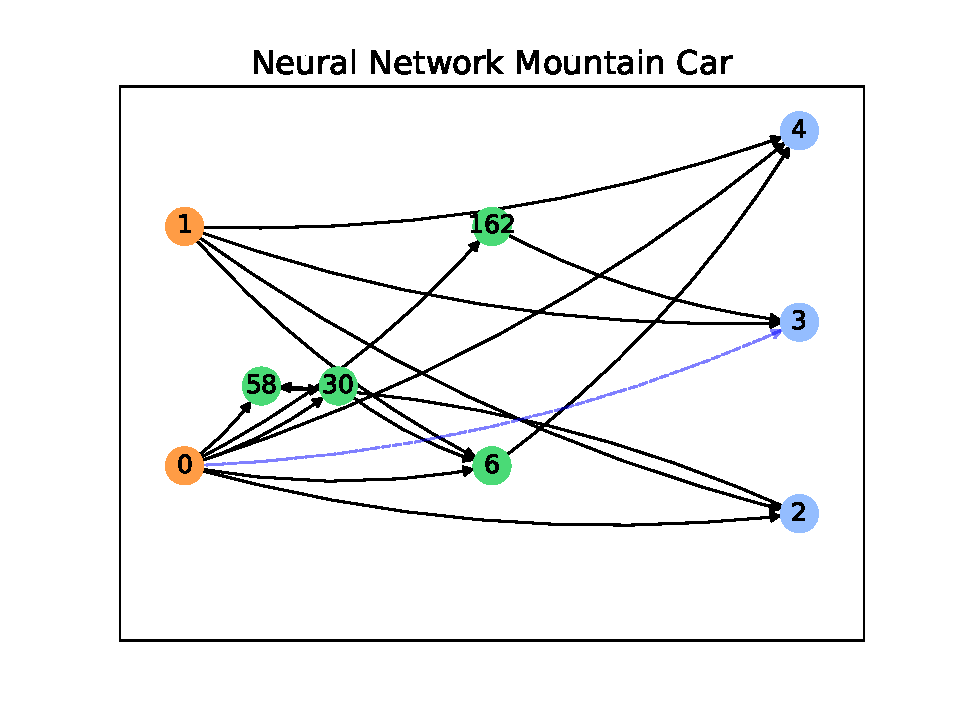
\includegraphics[width=1.0\textwidth]{./img/mountain_car_single/mountain_car_neural_network.pdf} 
	\end{minipage}
	\hfill
	\begin{minipage}[]{0.49\textwidth}
		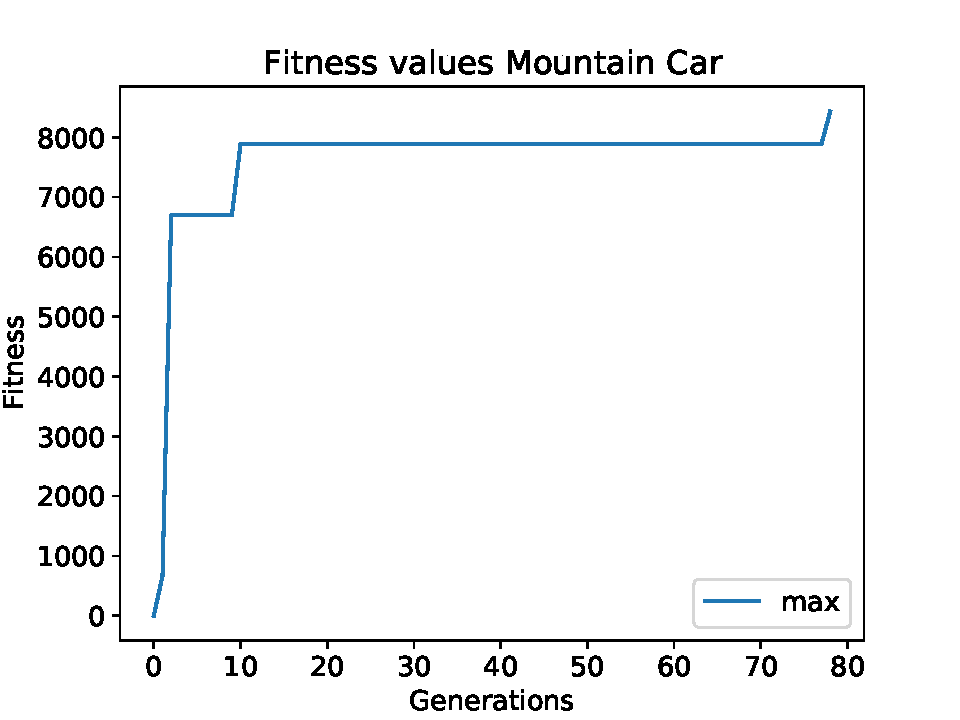
\includegraphics[width=1.0\textwidth]{./img/mountain_car_single/1413_fitness_1core_1pi.pdf} 
	\end{minipage}
	\caption{Links die Lösung für das Mountain Car Problem, rechts die dazugehörigen Fitnesswerte pro Generation mit 10 Prozessen}
	\label{fig:mountain_car_10core_neural_network_and_fitness}
\end{figure}
\\\\

\begin{figure}[!h]
	\centering
	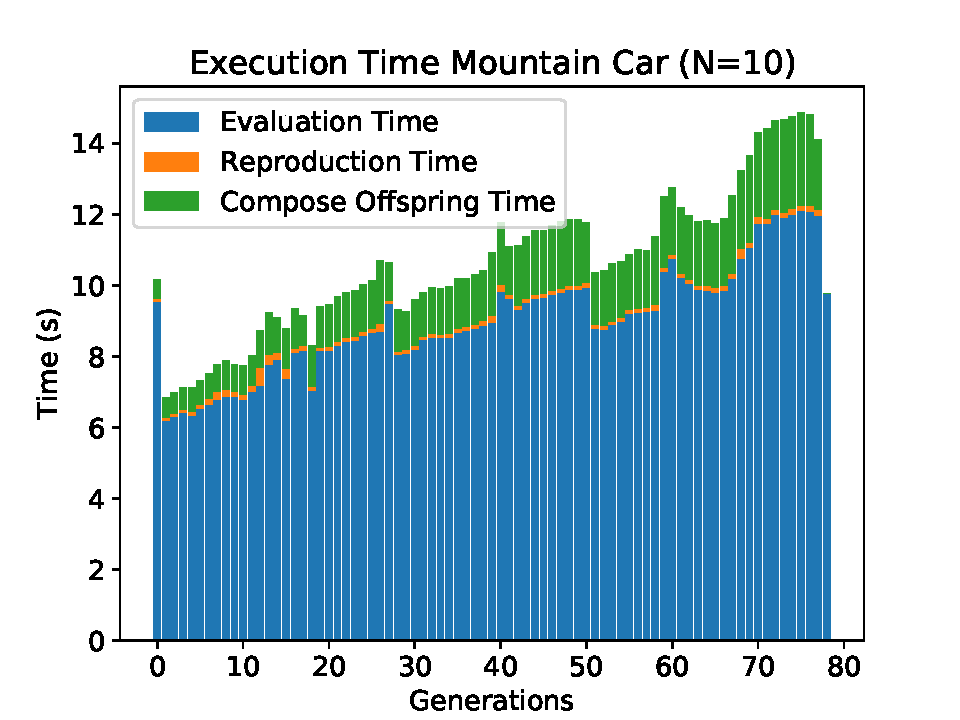
\includegraphics[width=0.5\textwidth]{./img/mountain_car_analysis/1413_time_10cores_10pis.pdf} 
	\caption{Ausführungszeit des \emph{Mountain Car} Problems auf mit 10 Prozessen }
	\label{fig:mountain_car_time_10cores_10pi}
\end{figure}

Im ersten Durchlauf wird der parallelisierte Algorithmus mit zehn Prozessen auf den zehn Raspberry Pis ausgeführt. Das Verfahren ist so konfiguriert, dass auf jeden Raspberry Pi ein Prozess gestartet wird.


% Zuerst Ergebnisse 10 Pis, mit Verifizierung Funktionalität und allgemeines Ergebnis
% Eingehen dass Master Pi keine Abarbeitugn übernimmt sondern nur Koordination
% Zeiten von anderen Phasen weichen ab, daher kann es zu varianzen kommen
% Allgemeine Laufzeit des Verfahrens und Laufzeit des evaluierten Verfahren anzeigen
% Vergleich mit Amdahls Law?

%In diesem Kapitel wird die parallelisierte Implementierung anhand der \emph{Mountain Car} und \emph{Pendulum} Umgebung evaluiert. Die gemessenen Ausführungszeiten werden dann mit denen der sequenziellen Implementierung verglichen und die Effizienz der Parallelisierung bewertet. Hierbei ist darauf zu achten, dass beide Implementierungen zu jederzeit dieselben Zwischenergebnisse liefern, sodass keine Implementierung einen Vorteil durch kleiner \ac{KNN} oder kürzere Evaluationszeiten hat. Für die Umsetzung hiervon wird sowohl die Implementierung und als auch die Konfiguration von \ac{NEAT} aus dem Kapitel \ref{sec:analysis_optimzation_problems} unverändert übernommen. Beim Ausführen des Optimierungsverfahren wird zusätzlich derselbe \emph{Seed} für jede Umgebung verwendet. Ist das parallelisierte Verfahren entsprechend den Anforderungen umgesetzt wird


%Sowohl die Implementierung des Optimierungsproblems als auch die Konfiguration von \ac{NEAT} werden aus Kapitel \ref{sec:analysis_optimzation_problems} übernommen. Ist das Verfahren entsprechend den Anforderungen durch einen \emph{Seed} konfigurierbar, sollten die Ergebnisse beider Implementierungen identisch sein.